%=========================================================================
% (c) 2011, 2012 Josef Lusticky

\chapter{Hardware real-time support}
\begin{figure}
	\centering
	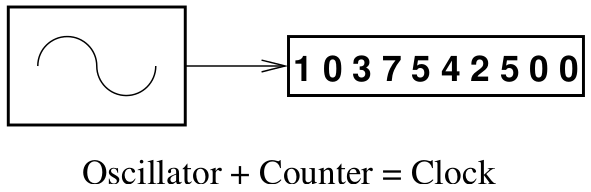
\includegraphics[width=6cm,keepaspectratio]{fig/clock.png}
	\caption{Clock by P. Kamp}
	\label{fig:hw-clock}
	%\bigskip
\end{figure}
For keeping, measuring and resolving time computer needs a clock.
Computer clock is an electronic device that counts oscillations in a
quartz crystal oscillator with a particular frequency~\cite{thesis-sync}.
These clocks are essentially timers associated with a counter register and
are capable of generating hardware interrupts.
The counter register counts the oscillations of the crystal.
When the counter registers reaches a specific value,
an interrupt is generated.
Such interrupt is called a {\it{clock tick}} (or {\it{timer tick}}) and at each clock tick,
interrupt service routine increments a system clock value stored in memory~\cite{thesis-sync}.
In a typical computer clock design, interrupts are produced at
fixed tick intervals in the range 1-20~ms~\cite{nanokernel}.
In recent years, however, a new design called {\it{tickless}} or {\it{dynamic ticks}}
has been in development~\cite{kernel-timer-systems}.
This allows an operating system kernel to run without a regular timer tick.
Such design is not used by Contiki OS~\cite{contiki-docs} and
therefore not further discussed in this thesis.


A typical desktop computer today includes CPU based on Intel x86 architecture.
Real-Time Clock (RTC) in CMOS memory that is battery powered

Unfortunately Intel x86 architecture is heavily influenced by backward compatibility,
and many hardware configurations are in use today -
e.g. the time value can also be stored in Binary Code Digit (BCD) encoding in RTC.

In year 19xx /, Starting with Intel 386,
Intel introduced
Programmable Interrupt Controller (PIT) Intel 8253 and 8254 - 3 counters (counter 0 interrupt to OS)

The problem with this device is that it only has
8bit bus-width, so reading a 16 bit timestamp takes
3 I/O operations: one to latch the count in an internal register,
and two to read the high and low parts
of that register respectively~\cite{timecounters}.
Obviously, on multi-CPU systems this cannot be
done without some kind of locking mechanism
preventing the other CPUs from trying to do the
same thing at the same time~\cite{timecounters}.


Used by historic versions of Linux
=> read initial time from RTC, setup PIT and interrupts (IRQ 0, INT 8), increment jiffies on every interrupt, provide application resolution of jiffies

init/main.c - time\_init() - read from RTC and save to startup\_time
kernel/sched.c - sched\_init() = PTI setup for interrupts - LATCH (1193180/HZ)
kernel/system\_call.s - timer\_interrupt() in assembly - increments jiffies

The current real time is provided by CURRENT\_TIME (startup\_time+jiffies/HZ) => since jiffies is integer and HZ is 100 => resolution of 10ms.
kernel/sys.c - sys\_time() - CURRENT\_TIME returned

\section{Interrupts}
Older x86 processors used an interrupt mechanism to switch from
user-space to kernel-space, but new x86 processors provide instructions
that optimize this transition (using sysenter and sysexit instructions)~\cite{ibm-linux-system-calls}.


TICK - http://www.ntp.org/ntpfaq/NTP-s-sw-clocks-tick.htm


- software:
The Kernel Discipline =  kernel clock model RFC 1589

However, some clock implementations do not allow small corrections to be applied to the system clock, and there is no standard interface to monitor the system clock's quality.
=> divide problem (in RFC)

\section{Clock quality factors}
The smallest possible increase of time the clock model allows is called {\it{resolution}}~\cite{ntp-faq}.
If a clock increments its value only once per second, its resolution is also one second.

A high resolution does not help anything if the clock can not be read.
Therefore the smallest possible increase of time that can be experienced
by a program is called {\it{precision}}~\cite{ntp-faq}.

When repeatedly reading the time, the difference may vary almost randomly.
The difference of these differences (second derivation) is called {\it{jitter}}~\cite{ntp-faq}.

A clock not only needs to be read, it must be also set.
The {\it{accuracy}} determines how close the clock is to an official time reference like UTC~\cite{ntp-faq}.

Unfortunately all the common clock hardware is not very accurate.
This is simply because the frequency that makes time increase is never exactly right.
Even an error of only 0.001\% would make a clock be off by almost one second per day~\cite{ntp-faq}.
It is sometimes convenient
to express frequency offsets in parts-per-million~(PPM), where~1~PPM
is equal to $10^{-6}$ $\frac{s}{s}$ (0.0001\%)~\cite{rfc5905}.
Real clocks have a frequency error of several PPM quite frequently
and some of the best clocks available still have errors of about $1^{-8}$PPM~\cite{ntp-faq}.

Even if the systematic error of some clock model is known, the clock will never be perfect.
This is because the frequency varies over time, mostly influenced by temperature,
but it could also be air pressure or magnetic fields, etc.
{\it{Reliability}} determines the time a clock can keep the time within a specified accuracy~\cite{ntp-faq}.

For long-term observation one may also notice variations in the clock frequency.
The difference of the frequency is called {\it{wander}}~\cite{ntp-faq}.
Therefore there can be clocks with poor short-term stability, but with good long-term stability, and vice versa.

The difference between the time reported by a clock and the
is called {\it{offset}}~\cite{thesis-sync}.
